\documentclass[runningheads]{llncs}

\usepackage{graphicx}
\usepackage{mathtools}
\usepackage{amsmath}
\usepackage{amsfonts}
\usepackage{hyperref}
\usepackage{xcolor}
\usepackage[T1]{fontenc}
\usepackage{fontspec}
\usepackage{listings, listings-rust}
\usepackage[skip=5pt plus1pt, indent=10pt]{parskip}
\usepackage{wrapfig}
\usepackage{float}
\usepackage{subcaption}
\usepackage{dirtree}

\raggedbottom

\setmonofont{Noto Sans Mono}[Scale=0.85]
\lstset{language=Rust, basicstyle=\ttfamily, float, floatplacement=H}

\hypersetup{
    colorlinks,
    linkcolor={blue!80!black},
    citecolor={blue!80!black},
    urlcolor={blue!50!black}
}

% \input{commands}

% \makeatother

% \input{unicode}

\title{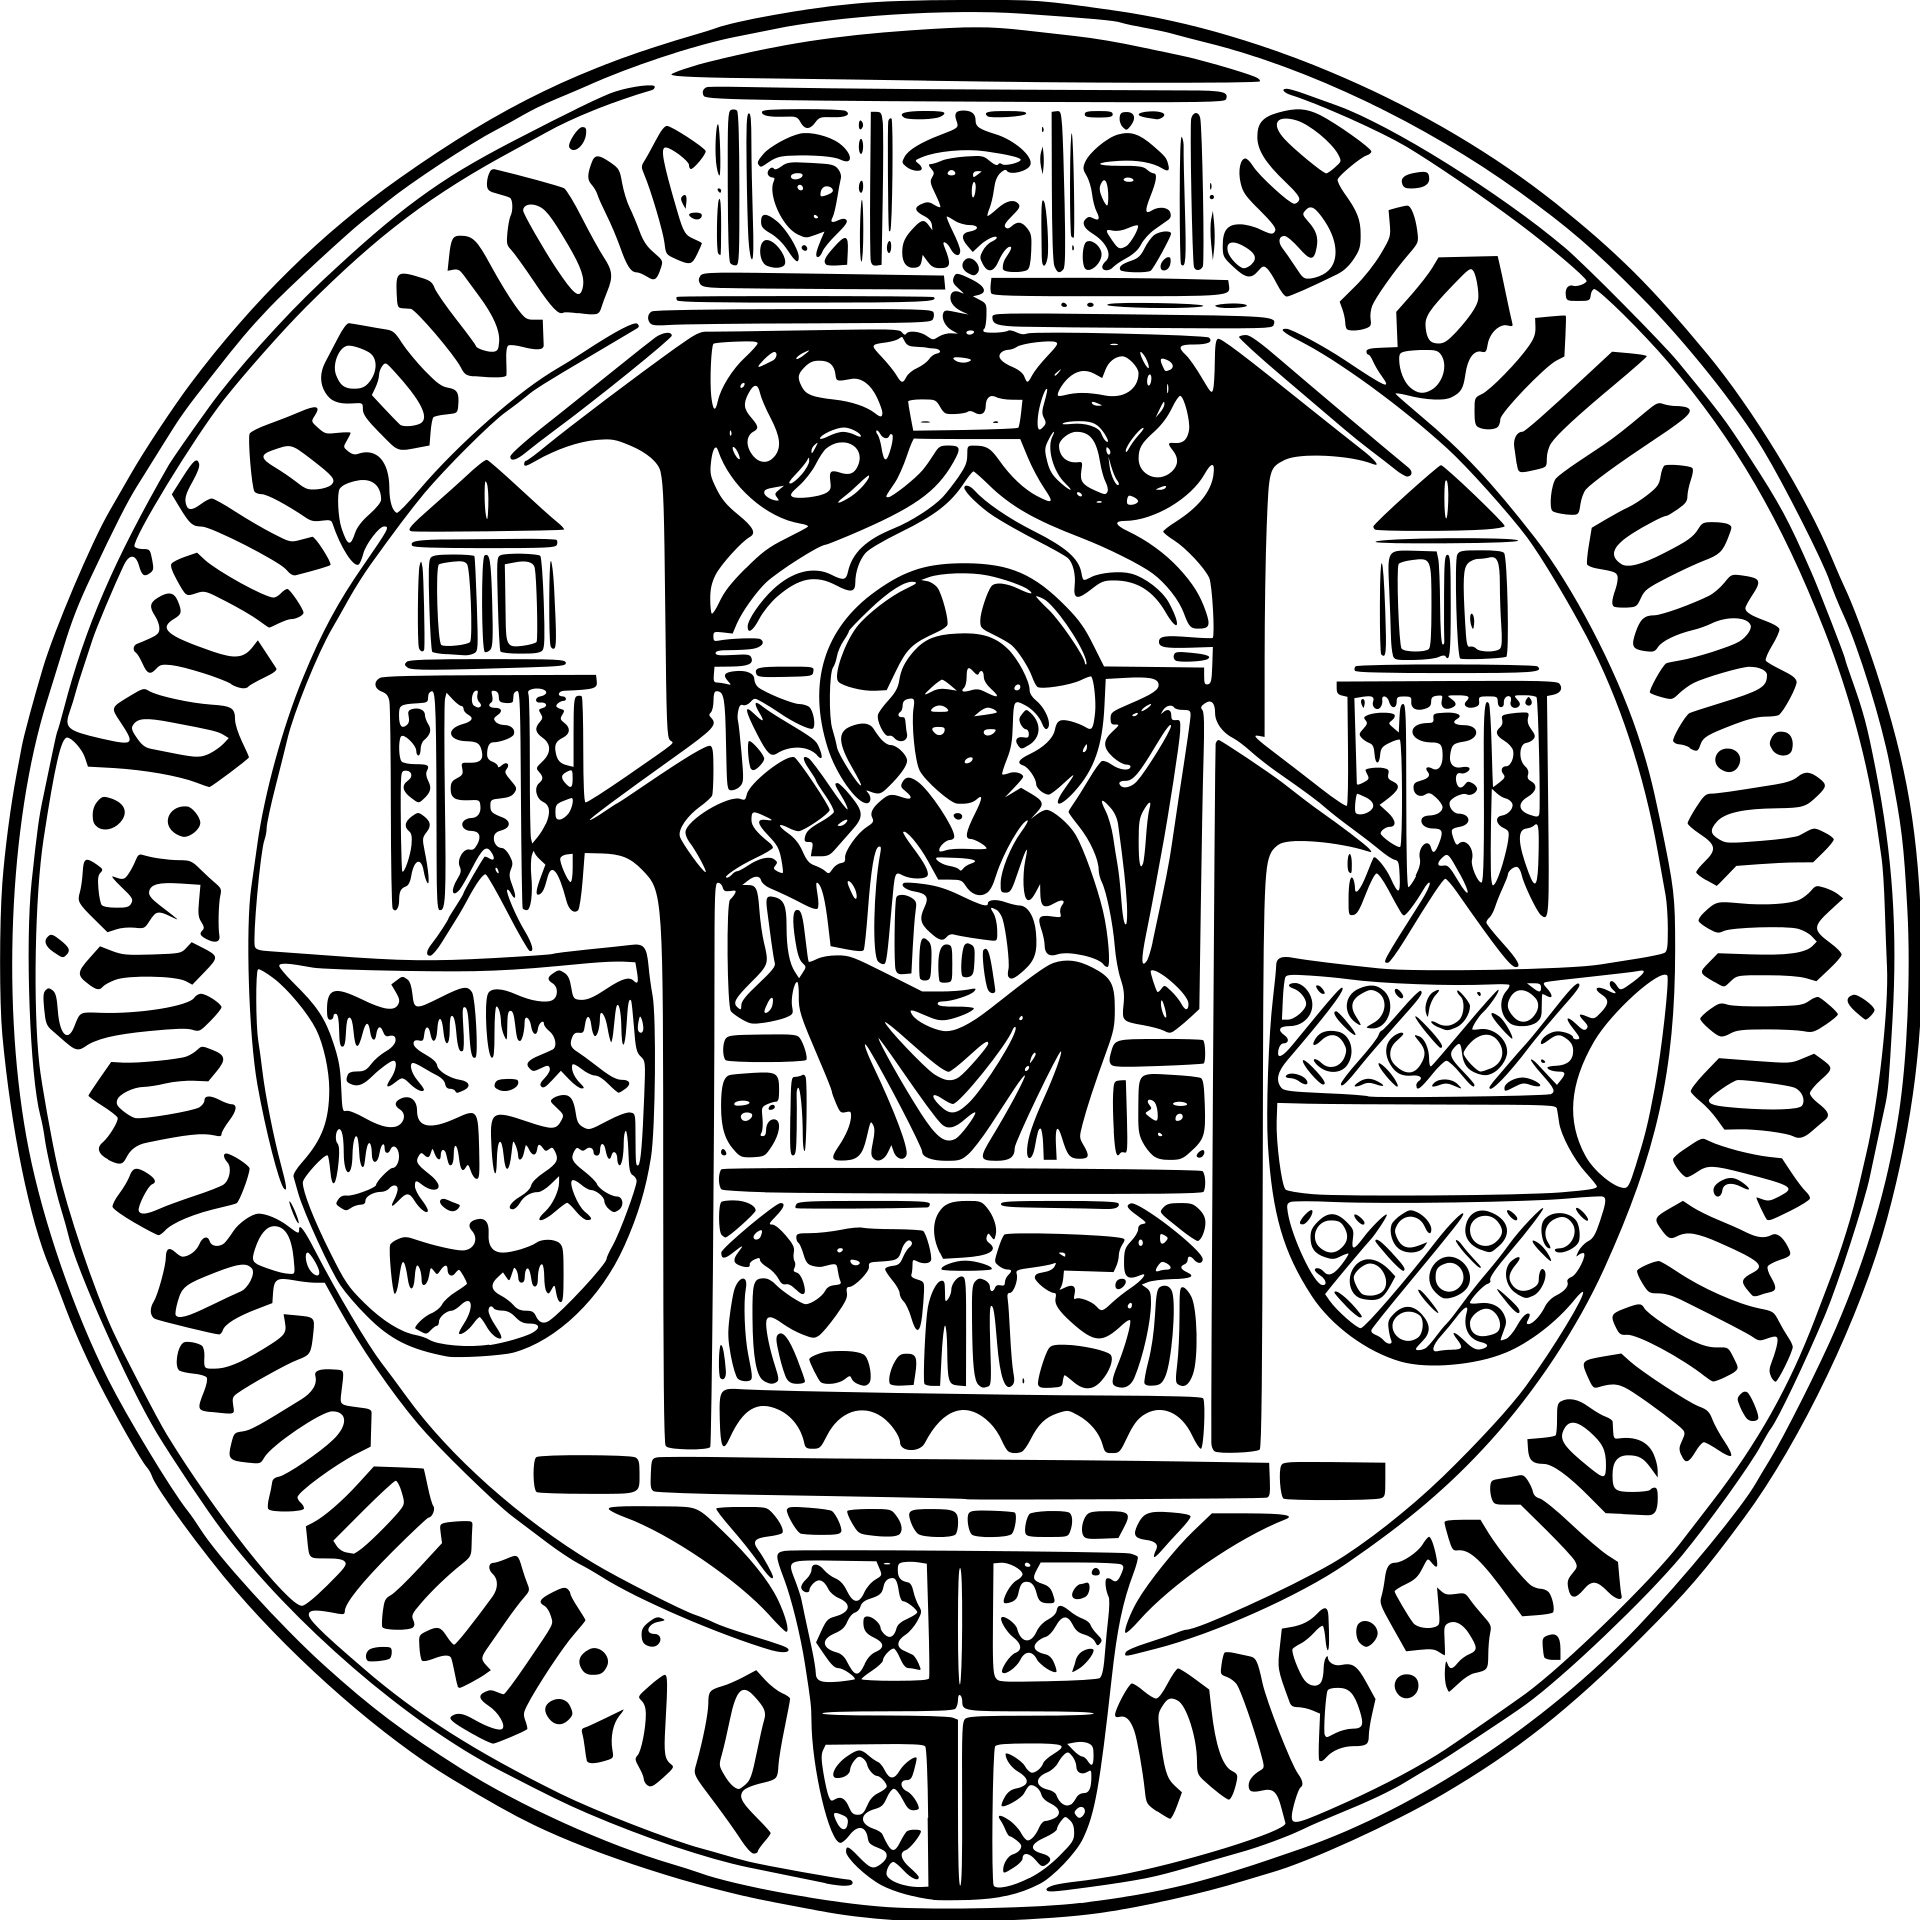
\includegraphics[width=0.4\textwidth]{logo.png}~ 
\\[1cm]
Embedded Probabilistic Programming in Rust}
\titlerunning{Embedded Probabilistic Programming in Rust}
\institute{Chair of Programming Languages, University of Freiburg}
\author{Tobias Hoffmann\\\email{garbaz@t-online.de}}
\authorrunning{T. Hoffmann}


\begin{document}

\let\oldaddcontentsline\addcontentsline
\def\addcontentsline#1#2#3{}
\maketitle
\def\addcontentsline#1#2#3{\oldaddcontentsline{#1}{#2}{#3}}


\noindent\makebox[\linewidth]{\bf{Bachelor Thesis}}
\\

\noindent\makebox[\linewidth]{Examiner: Prof. Dr. Peter Thiemann}
\noindent\makebox[\linewidth]{Advisor: Hannes Saffrich}

% \input{SystemF}
% \input{SystemFo}
% \input{DictionaryPassingTransform}

\begin{abstract}
  The paradigm of probabilistic programming allows for the expression of computationally arbitrary generative probabilistic models and provides general model-independent inference algorithms over them. This paper presents and overview over the theory behind one particular commonly employed inference algorithm, the Metropolis-Hastings algorithm, how it can be applied to probabilistic programs, and an implementation of a probabilistic programming framework embedded into the imperative programming language Rust.
\end{abstract}
\begin{abstract}\textbf{(Deutsch)}
  Das Prinzip probabilistischer Programme erlaubt einem das Formalisieren rechnerisch beliebiger generativer probabilistischer Modelle und bieten allgemeine modellunabhängige Inferenzalgorithmen für diese. Diese Arbeit präsentiert einen Überblick über einen häufig verwendeten Inferenzalgorithmus, den Metropolis-Hastings-Algorithmus, wie dieser angewandt werden kann auf probabilistische Programme, und eine Implementierung eines Frameworks für eingebettete probabilistische Programme in der imperativen Programmiersprache Rust.
\end{abstract}

\setcounter{tocdepth}{2}
\tableofcontents
\newpage 

\section{Introduction}

For various systems across many fields of interest, randomness can be useful in developing tractable models by abstracting over the dynamics of some complex process, such as for example the physics of a coin flying through the air being abstracted over with a simple Bernoulli distribution to model it's behavior of either landing on heads or tails. Unlike different methods of abstraction, like approximate simulation, if constructed accurately, a distribution can precisely capture a part of the behavior of a system without having to fully reproduce it's internal mechanics. Specifically, while a single draw from a distribution will not necessarily match some observed behavior, the characteristics of a total of draws will approach the characteristics of an equal number of independent observations.

While there are many examples of the behavior of principally rather complex systems being well approximated by mathematically simple distributions, like for example the distribution of beans in a "bean machine" following a normal distribution, most systems of practical interest do not give rise to such easily describable distributions. Rather, to develop a stochastic abstraction over the mechanics of many systems requires the arbitrarily complex composition of simple distributions, to a point that it can become difficult or even impossible to analytically answer questions of interest about the resulting total distribution. For example, while it might be easy to directly calculate the expected value or variance of some well understood distributions and even of simple combinations of distributions, like a linear combination of real-valued distributions, for many complex distributions this no longer is directly possible.

However, many characteristics about a complex distribution can still be approximated by a general category of methods called "Monte Carlo methods", which rather than analytically working on the structure of a distribution itself to obtain results instead compute numerical approximations by taking random samples from the distribution, just as one would statistically analyze observations from any process.

While it no longer is required for our target distribution to be fully analytically comprehensible to apply a Monte Carlo method of approximation, it is crucially still necessary to have the means to obtain a large number of samples from our distribution, which itself can already be rather difficult to develop for many complex distributions. Though while it might be difficult to generate samples, often times it is much easier to at least compute the probability of some given value having been drawn from a certain distribution.

To still obtain samples under such relaxed conditions, where the only practically computable function is getting the probability of some value being drawn from the distribution, a class of algorithms collectively called "Markov Chain Monte Carlo methods" (MCMC) have been developed. The principle operation of these methods is to iteratively explore the space of values that might be drawn from a distribution by taking repeated randomized steps through it and for each step deciding whether to take it or to revert back to the previous value. If the method of proposing steps to take and deciding whether to accept or reject them is chosen correctly, the resulting sequence of values will converge to a distribution which matches the target distribution. This way we can generate samples from a distribution without having to actually be able to directly draw such samples, allowing us to use Monte Carlo methods to get approximations for characteristics of interest about our distribution.

While MCMC methods are widely used in various fields of application, such as physics, economics and many other endeavors of both academia and industry, and routinely applied to potentially very high-dimensional and complex stochastic models, these usually are still drawn from a computationally significantly constrained class, such as generalized linear models. We will here consider a much wider class of models, that of probabilistic programs.

For our purposes, we will consider a probabilistic program to be a function in a Turing-complete imperative programming language which can contain two additional elements besides the language's regular semantics: Instances of sampling from predefined primitive distributions or other probabilistic programs, and statements of observing some value from some primitive distribution.

Introducing randomness into an otherwise deterministic program is itself not much of a significant change to the execution model of a programming language with persistent state, with most everyday programming languages having some readily provided means of getting random, or at the least pseudo-random, values for various practically relevant distributions. So without any change to execution, we can model many computationally complex distributions by simple writing some function which utilizes such primitive distributions. Drawing samples from the composite distribution then corresponding to simply executing this function.

However, in many practical tasks, we might not simply want to obtain some value from a distribution and run with it, but rather wish to express a constraint on such a value. For a very common example, we might have some complex stochastic model, written as a probabilistic program, and some empirical observations of data from some real-life system we wish to understand, and want to know which instances of of our model reproduce most closely this data.

One straightforward possibility would be to simply run our program many times and reject samples which do not fit the observed data. This is called "rejection sampling" and is for relatively simple models with a finite and relatively small space of possible output values a feasible method, if however perhaps computationally somewhat wasteful. But for any more complex model, and especially for distributions over a non-finite domain, this method is infeasible. Rather, an approach which more efficiently explores the possible executions of a probabilistic program is necessary.

To solve this problem with MCMC methods, three considerations have to be made: What is the space over which we define our distribution which we will explore? How will we be able to compute the probability of some sample coming from our distribution? How will we efficiently step through this space while also fulfilling the constraints necessary for our algorithm to efficiently sample from the target distribution?

While there any many answers to the final of these three questions, the first two have relatively straightforward solutions. The space we will explore with MCMC is the space of possible executions of a probabilistic program at hand, more specifically the space of traces of draws from primitive distributions throughout it. And to calculate the probability of some particular trace being a possible execution of the program, we simply run the program and accumulate the probabilities of the individual draws and observations of values from primitive distributions as we encounter them during execution.


% \section{Probability Theory}

\section{Markov Chains}

A Markov chain is a random sequence of values from some space. In contrast to any other random sequence, a Markov chain is characterized the particular property that the distribution determining every value in the chain is dependent on exactly the directly preceding value. If considered as a series of steps through some space of values, this means that every step taken is only based on the current location in the space, and entirely agnostic to how we got there. Or perhaps more philosophically, in a Markov chain, the future depends on the present, but not the past.

In mathematical terms, we define a \textit{Markov chain} as a series $(x_t)_{t \in \mathbb{N}_0}$ in some space $\mathbb{X}$, where we choose the starting value $x_0$, and every value $x_{t + 1}$ after that is defined in accordance to some \textit{transition kernel} $k$, $x_{t+1} \sim k[x_t]$.

The advantage of such a forgetful sequence is that it is possible to prove general propositions about it's behavior, such as whether or not it will converge towards a stable distribution and what this distribution will look like. But by each value depending on the previous, much more interesting behavior can emerge than with a sequence of entirely independently drawn samples.

While Markov chains are often times conceptualized as a directed graph consisting of nodes representing the possible states the chain can jump between at each step, and weighted edges representing possible transitions between states with their relative probability, for our purposes it is more useful to consider a Markov chain as a series of time-discrete steps in some, potentially high-dimensional and highly structured, abstract space of values.

At each point in time therefore we are at some value and make a decision as to which value to jump to next. The choices of these incremental decisions will accumulate to determine the properties of the resulting sequence of values.

As a tangible example, one might consider the one dimensional array of integer numbers, where at each step we throw a coin to determine whether to take a step in the negative direction or a step in the positive direction. Or for another example perhaps a two dimensional space of real-numbered pairs and a walk throughout it where at each step a value from a two dimensional normal distribution is draw to determine in what direction and how far to jump next. In either case, the result will be a random sequence of values characterized by both the space they came from and the random distribution by which we stepped through this space.

The core property of Markov chains that is of interest for our purposes is that, if the transition kernel satisfies certain properties, the series $(x_i)_{i \in \mathbb{N}}$ will stochastically converge to a certain \textit{equilibrium distribution} $p_eq$ \cite{bonawitz2008composable}, meaning that the series will for higher and higher $t$ tend to look more and more as if each value $x_t$ was simply drawn from $p_eq$.


\section{Metropolis Hastings}

While there are many Markov chain Monte Carlo algorithms (MCMC), with differing conditions for application and advantages/disadvantages in terms of implementation complexity and performance, we will focus here on a principally rather simple algorithm, the "Metropolis-Hastings algorithm" (MH) \cite{metropolis1953equation} \cite{hastings1970monte}.

The problem we are trying to solve with MH is obtaining representative samples from some distribution of interest $\pi$, the \textit{target}, for which we only are able to compute the probability density $\pi(\cdot)$. And as is the principle of MCMC methods, we do so by exploring the space $\mathbb{X}$ of possible samples from $\pi$, its \textit{support}, via the iterative development of a Markov chain through this space. How exactly these steps are taken is the principal concern of MH.

To apply MH to sampling from some distribution $\pi$, we first need to pick a (usually, relative to $\pi$, very simple) distribution $q[x]$, the \textit{proposal kernel}, with the same support as $\pi$. This kernel defines our exploration of the support $\mathbb{X}$. Specifically, at every step $x_t$ in our Markov chain we use $q$ to choose a possible next step $\hat{x}_{t+1} \sim q[x_t]$. So $q$ can, and usually will, depend on the current position $x_t$ in $\mathbb{X}$.

If our $\pi$ were for example defined over $\mathbb{X} = \mathbb{R}^2$, a possible candidate for $q$ would be a two-dimensional normal distribution centered around $x_t$. So at each step in the Markov chain exploration of $\mathbb{X}$, we would draw $\hat{x}_{t+1} \sim \mathcal{N}^2[\mu = x_t, \sigma^2]$ (with $\sigma^2$ being a parameter to be tuned for faster convergence).

If we were to simply always take this proposed step $\hat{x}_{t+1}$ drawn from $q[x_t]$, then the result would be a random walk through $\mathbb{X}$ entirely independent from our target distribution $\pi$. With the goal of course being to obtain a series of samples from $\pi$, this would not be of much use.

The second part to every sampling step in the MH algorithm is to decide whether to take the proposed step drawn from $q[x_t]$, $x_{t+1} := \hat{x}_{t+1}$, or whether to remain at the current position in $\mathbb{X}$, $x_{t+1} := x_t$. This decision is itself done randomly:

\begin{align*}
x_{t+1} & = \begin{cases}
    \hat{x}_{t+1} & \text{ if } u \le \alpha \\
            x_{t} & \text{ otherwise }
            \end{cases} \\
\alpha & = \frac{\pi(\hat{x}_{t+1})}{\pi(x_t)} \frac{q(x_t | \hat{x}_{t+1})}{q(\hat{x}_{t+1} | x_t)} \\
u & \sim \mathcal{U}[0,1]
\end{align*}

The value $\alpha$ defined here is called the \textit{acceptance ratio}. If $\alpha$ is equal to $0$, say if $\pi(\hat{x}_{t+1}) = 0$, then we will definitely remain in place, since $P(U \le 0) = 0$. So our Markov chain will never step to values which are impossible to be a sample from $\pi$.

If on the other hand $\alpha$ is greater than or equal to $1$, say if $\pi(\hat{x}_{t+1}) \ge {\pi(x_t)}$ and $q(x_t | \hat{x}_{t+1}) = q(\hat{x}_{t+1} | x_t)$, then we will definitely take the proposed step, since $P(U \le 1) = 1$. So our Markov chain will always tend towards regions of more likely values under $\pi$.

For any $\alpha$ between $0$ and $1$, we will sometimes take the proposed step and sometimes will not, depending on what value is drawn for $\mathcal{U}[0,1]$. So we can still step "back down" to values that are less likely than the current value, but this is increasingly unlikely the smaller the ratio between the probability under $\pi$ of the value after a proposed step and of the current value. As a result, we will generally tend towards sampling from regions of high probability under $\pi$, while also in the long run exploring regions of lower (non-zero) probability.

And under some assumptions about the target distribution $\pi$ and the kernel $q$ it is possible to rigorously prove that, at least in the limit, the Markov chain of samples generated as such will eventually converge to being a sequence of (dependent) samples from $\pi$ \cite{metropolis1953equation}.

So in total the complete Metropolis-Hastings algorithm looks as follows:

\begin{minipage}{\linewidth}
\begin{itemize}
\item Repeat forever:
  \begin{itemize}
  \item Sample $\hat{x}_{t+1}$ from $q(x_t)$
  \item Calculate acceptance ratio $\alpha$ based upon $\hat{x}_{t+1}$ and $x_t$
  \item Sample $u \sim \mathcal{U}[0,1]$
  \item If $u \le \alpha$, then $x_{t+1} := \hat{x}_{t+1}$, else $x_{t+1} := x_t$
  \end{itemize}
\end{itemize}
\end{minipage}

One in practice often times highly relevant property to note about the definition of MH is the fact that we only ever need to compute a ratio $\frac{\pi(x)}{\pi(y)}$ between two results of the probability density function $\pi(x)$. This means that we do not actually have to be able to compute $\pi(x)$ directly, but rather that it is sufficient to be able to compute some proportional function $\tilde{\pi}(x) \propto \pi(x)$, since $\frac{\tilde{\pi}(x)}{\tilde{\pi}(y)} = \frac{\pi(x)}{\pi(y)}$.

As a very common practical example, say we would like to generate samples from some posterior distribution:

\begin{equation*}
\pi(x) = p(x | w) = \frac{p(w | x) p(x)}{p(w)}
\end{equation*}

While calculating $p(w | x)$ and $p(x)$ might be straightforward, often times directly getting a value for $p(w)$ is rather difficult. Usually one would have to compute it from the other two quantities as $p(w) = \int p(w | x) p(x) dx$.

With MH however, since $p(w)$ does not depend on $x$ and we only need to know $\pi(x)$ up to a proportionality constant, we can simply define $\tilde{\pi}(x) = p(w) \pi(x) = p(w | x) p(x)$ and calculate our acceptance ratio $\alpha$ with respect to $\tilde{\pi}$ rather than $\pi$, sidestepping the need to evaluate any possibly intractable integrals.


A probabilistic program for the purposes of our implementation here is syntactically simply an ordinary function in an (in our case imperative) programming language. This function can contain any code constructs that are part of the host language, including potentially troublesome things like conditionals, loops and recursion. However, a probabilistic program can, as opposed to an ordinary function, contain two additional syntax elements: "sample" expressions and "observe" statements.

Besides the syntactic difference to an ordinary function, the execution of a probabilistic program also differs in a significant way. In addition to running the code as normal, during execution track is kept of what distributions are sampled from with what parameters, what values are drawn and how probable the drawing of these values was, and most importantly, the total probability of the particular execution happening. This trace of the probabilistic programs execution allows for the application of inference algorithms, as will be detailed later on.

\subsection{Sample Expression}

A sample expression is semantically rather simple, it allows us to sample a value from some distribution, be it a primitve distribution provided by our implementation or a distribution defined as another probabilistic program. For the regular semantics of the program the resulting value of a sample expression is in every regard no different than as if it were simply an ordinary function call. However, upon a sample expression being encountered during execution it is recorded to the execution's trace what distribution has been sampled from with what parameters, what value has been drawn, and how likely it was for this value to come from the distribution.

\begin{minipage}{\linewidth}
\begin{lstlisting}
/// Sampling from a primitve distribution and using recursion
#[prob]
fn example1(p : f64) -> u64 {
    let c = 0;

    while sample!(bernoulli(p)) {
        c += 1;
    }

    c
}
\end{lstlisting}
\end{minipage}

\begin{minipage}{\linewidth}
\begin{lstlisting}
/// Sampling from another probabilistic program and using
/// conditionals & recursion
#[prob]
fn example2(n : u64) -> u64 {
    if sample!(example1(1./(n as f64))) >= n {
        0
    } else {
        1 + sample!(example2(n))
    }
}
\end{lstlisting}
\end{minipage}


\subsection{Observe Statement}

The other special kind of expression we can use in a probabilistic program is an `observe` statement. It allows us to state that, at this position in the code, and therefore possibly dependent on values computed so far, we "observe" some value from some distribution. We essentially say that "we know that this value is the result of sampling from this distribution", which might or might not be likely, correspondingly affecting the probablity of the final value resulting from the probabilistic program as a whole. 

Neither the value we are observing, nor any parameters to the distribution have to be constant. They can result from any arbitrary combination of ordinary and probabilistic computations. However, we can not observe values from a distribution defined by another probabilistic program, only from primitive distributions.

Observing a value from a distribution does not have any direct effect on the execution of our program. If we were to take a probabilistic program and remove all observe statements, it would still principally run the same way. However, observe statements greatly affect the way samples are drawn from the probabilistic program, specifically the total probability of the current execution. If for example, we were to observe a value of $2$ from a uniform distribution $\mathcal{U}(0,1)$, which of course is not possible, i.e. has a probability of zero, then the total probability of the execution would also be zero. In short, observe statements allow us to, smoothly, constrain what instances of our model are likely or even possible.

\begin{minipage}{\linewidth}
\begin{lstlisting}
/// What parameter `p` for a bernoulli distribution explains our
/// observed results best?
#[prob]
fn example3(obs : [bool]) -> f64 {
    let p = sample!(uniform(0., 1.));

    for o in obs {
        observe!(o, bernoulli(p));
    }

    p
}
\end{lstlisting}
\end{minipage}

\begin{minipage}{\linewidth}
\begin{lstlisting}
/// What might have been the start position of a random walk,
/// given we know the end position and the number of steps?
#[prob]
fn example4(steps : u64, end_pos : f64) -> f64 {
    let start_pos = sample!(uniform(-10.,10.));
    
    let mut pos = start_pos;
    for _ in 0..steps {
        pos += sample!(normal(0.,0.5));
    }
    
    observe!(end_pos, normal(0.,1.));

    start_pos;
}
\end{lstlisting}
\end{minipage}


\subsection{Condition Statement}

While the core semantics of probabilistic programs are fully described by the addition of sample and observe statements, in practice we often times don't just want to observe some value from some distribution, but rather want to put a hard constraint on what executions should produce valid samples, and what shouldn't. A condition statements allows us to do just that. It checks whether some arbitrary boolean expression evaluates to $\text{true}$, and if it doesn't, the probablity of the whole execution is set to $0$. Otherwise, it does nothing.

Just like with the observe statment, the condition statement doesn't interfer at all with the regular execution of the program, but rather only affects the calculation of the total probablity. So in the end, even if the expression inside a condition statement evaluates to $\text{false}$, the function will continue as normal and still return a value as normal, but the associated probablity is $0$.

In fact, the effect of a condition statement is no different from an observe statement with the value of the boolean expression being observed from a distribution from which we sample the value $\text{true}$ with a probablity of $1$, like for example a Bernoulli distribution $\text{Bern}(p)$ with a parameter of $p=1$. However, in pratice, both for readability and a small increase in computational efficiency, we rather use a condition statement directly to express hard constraints on the execution of our probabilistic program.

It should be noted however, that, whenever possible, we should try to soften any hard conditions in our program to observes, to allow for executions that don't quite satisfy our constraints to have non-zero probablity. Otherwise, there is no way for the inference algorithm to know whether a sample from the program has a probablity of 0 because it's completely off from being from a valid execution or very close but just not quite there, causing the algorithm to devolve into a rejection sampler, which greatly impacts efficiency.

In the following we will only concern ourselves with sample expressions and observe statements, since condition statements are just a particular kind of observe statement.

\begin{minipage}{\linewidth}
\begin{lstlisting}
/// Modelling heights of e.g. people with a normal distribution
/// around some mean value.
/// However, a person's height can never be negative!
#[prob]
fn example5(mean_height : f64, deviation : f64) -> f64 {
    let height = sample!(normal(mean_height, deviation));
    condition!(height > 0);
    height
}

/// Instead of the condition expression, we could also simply
/// observe the value of our expression from a `bernoulli(1.)`
/// distribution.
#[prob]
fn example5b(mean_height : f64, deviation : f64) -> f64 {
    let height = sample!(normal(mean_height, deviation));
    observe!(bernoulli(1.), height > 0);
    height
}
\end{lstlisting}
\end{minipage}

\begin{minipage}{\linewidth}
\begin{lstlisting}
/// We can even simply define our own `condition` as a 
/// probabilistic program.
#[prob]
fn condition(c : bool) {
    observe!(bernoulli(1.), c);
}
\end{lstlisting}
\end{minipage}

\section{Trace Space}

If a probabilistic program at hand were only to contain sample expressions and no observe statements, drawing samples from the distribution represented by it would be as simple as just running the program as normal. However, if we were to do the same with a program that does contain observe statements, we would get samples that do not represent the actual distribution described by the program. We could even get samples which have a probability of $0$, simply by the execution resulting in that sample containing observe statement that are impossible. In general, a probabilistic program with observe statements does not directly function as a sampler for the distribution it represents. All it does is to produce random values and correctly calculate the probability of these values.

And that is not even enough to directly apply the Metropolis Hastings (MH) algorithm to the problem of getting representative samples from our program, since to explore some space with MH we need to be able to pick some arbitrary point in this space and ask for the probability of it coming from the distribution. So if we were to want to explore the space of values output by our probabilistic program, we would have to be able to pick some value and ask somehow how likely it would have been for it to return this value. This is not directly possible for any arbitrary probabilistic program.

However, there is a space for which our probabilistic program can answer this question necessary for applying MH, and that is the space of possible executions of the program. Rather than running our probabilistic program normally and actually drawing a random value at each sample expression, accumulating the total probability of the execution in the process, we instead pick the value to be drawn at every sample expression beforehand and then run the program, we still get the correct total probability for this execution, but for a \textit{trace} of predetermined values.

A trace of a probabilistic program is simply some representation of all the evaluations of sample expressions that are encountered during some particular execution of the program. This trace can contain a different number of entries for different executions, if for example the number of times a sample expression in a loop (or recursion) is encountered depends on a previous sample expression (Fig. \ref{example7}). And it can also be that the n-th sample expression we encounter during some execution is completely different from the n-th one we encounter during a different execution, if for example we were to sample from a normal distribution in one branch of an `if` and from a Bernoulli distribution in the other (Fig. \ref{example8}). So unfortunately "picking" some actually valid trace for a probabilistic program at hand is not straightforward. And even if we do have a valid trace, were we to make any changes to it, there is no certainty that the modified trace still represents a possible execution of the program.

% \begin{minipage}{\linewidth}
\begin{figure}[h]
\begin{lstlisting}
#[prob]
fn example7(p: f64) -> usize {
    if sample!(bernoulli(p)) {
        0
    } else {
        1 + sample!(example7(p))
    }
}
\end{lstlisting}
\caption{Depending on how many times we draw a \lstinline{false} from the Bernoulli distribution, a different number of sample expressions is encountered during an execution.}
\label{example7}
\end{figure}
% \end{minipage}


% \begin{minipage}{\linewidth}
\begin{figure}[h]
\begin{lstlisting}
#[prob]
fn example8() -> f64 {
    if sample!(bernoulli(0.1)) {
        if sample!(bernoulli(0.5)) {
            1.
        } else {
            -1.
        }
    } else {
        sample!(normal(0., 1.))
    }
}
\end{lstlisting}
\caption{Depending on whether we sample \lstinline{true} or \lstinline{false} from the Bernoulli distribution, the second sample expression we encounter could either be to again sample from a Bernoulli distribution or to sample from a normal distribution.}
\label{example8}
\end{figure}
% \end{minipage}

We therefore consider a trace of a probabilistic program not to necessarily be a one-to-one representation of a possible execution of the program. Rather, we allow for a trace picked beforehand for the execution of our program to only impose predetermined values for some of the sample expressions, and also to contain entries that are incorrect or are never reached. During execution, every time a sample expression is evaluated, we look into the trace and see if there is an entry determining what the result of the evaluation should be. If we do find an entry, we take the value, otherwise we just non-deterministically sample a new value and insert it into the trace as if it had always been there. Once the partially deterministic execution has completed, we discard any entries in the trace that weren't used, and so end up with a trace that once more represents a possible execution. A trace that fully determines the execution of our probabilistic program we call a \textit{valid} trace. It might contain unused entries, but it at least has to contain an entry for every sample expression encountered, making the execution fully deterministic.

Given that the parameters to a distribution can arbitrarily depend on the results of previous sample expressions, it is also very likely that the entry we find when trying to deterministically evaluate a sample expression is for the same distribution, but with different parameters (Fig. \ref{example9}). In this case, we can still deterministically use the value from the trace, but have to re-evaluate its probability under the distribution with the new parameters.

% \begin{minipage}{\linewidth}
\begin{figure}[h]
\begin{lstlisting}
#[prob]
fn example9(m : f64) -> f64 {
    let s = sample!(uniform(1., 10.));
    sample!(normal(m, s))
}
\end{lstlisting}
\caption{Depending on the value sampled from the uniform distribution the parameters for the normal distribution differ.}
\label{example9}
\end{figure}
% \end{minipage}

We can mostly treat sample expressions that sample from other probabilistic programs the same as ones that sample from primitive distributions. However rather than our trace containing a predetermined resulting value for the sub-program, it contains a predetermined sub-trace for it. We simply semi-deterministically run the sub-program on this sub-trace, possibly updating it along the way, just as we are doing for the main program. If the sub-program itself samples from another probabilistic program, we do the same there, and so on.

% \begin{minipage}{\linewidth}
\begin{figure}[h]
\begin{subfigure}{0.5\textwidth}
\begin{lstlisting}
#[prob]
fn flip() -> bool {
    sample!(bernoulli(0.5))
}

#[prob]
fn example10() -> f64 {
    let x = sample!(uniform(0., 10.));
    let y = if sample!(flip()) {
        sample!(normal(0., 1.))
    } else {
        sample!(uniform(-1., 1.))
    };
    x + y
}
\end{lstlisting}
\end{subfigure}
\begin{subfigure}{0.55\textwidth}
\dirtree{%
.1 example10.
.2 uniform(0,10) => 4.03 : 0.100.
.2 flip.
.3 bernoulli(0.5) => true : 0.500.
.2 normal(0,1) => -1.13 : 0.209.
}
\end{subfigure}
\caption{A probabilistic program that samples from another probabilistic program and an example trace for this program. Trace entries are formatted as \lstinline{distribution(parameters) => value : probability}.}
\label{example10}
\end{figure}
% \end{minipage}

Since the number of times any sample expressions appearing inside loops in our probabilistic program are encountered can depend on the value of prior sampling expressions, we also allot for every iteration of a loop a sub-trace, such that the number of times a loop is executed does not affect whether or not the entry in the trace corresponding to any sample expressions appearing after the loop is found or missed.

So formally, we define a trace as a tree $T := L(\mathbb{N}_0, [T]) | F(\mathbb{I}, [T]) | P(D,P,V)$ (Similar to Wingate et al.'s database \& naming scheme \cite{wingate2011lightweight}). A node $L(n,t)$ represents an iteration $n$ of a loop and its corresponding sub-traces $t$. A node $F(i, t)$ represents a sample expression sampling from another probabilistic program identified by some identifier $i$, and the corresponding sub-traces $t$. And a node $P(d,p,v)$ represents a sample expression sampling from a primitive distribution $d$ with parameters $p$, and the sampled value $v$.

We define the semi-deterministic evaluation $sdeval(f,t)$ of a probabilistic program $f$ for a given trace $t$ as follows:

\begin{minipage}{\linewidth}
% \begin{figure}[h]
\begin{itemize}
\item Execute $f$ as normal, but ...
  \begin{itemize}
  \item ... every time any kind of loop expression would be evaluated, do instead:
    \begin{itemize}
    \item Initialize a counter $c := 0$
    \item For every iteration of the loop:
      \begin{itemize}
      \item Look in $t$ whether a sub-trace for this iteration exists
      \item If it doesn't, create a new one and attach it to $t$
      \item Shadow $t$ to be this sub-trace for the scope of this iteration
      \item Run the body of the loop as normal
      \item Increment counter $c := c + 1$
      \end{itemize}
    \end{itemize}
  \item ... every time a sample expression would be evaluated, do instead:
    \begin{itemize}
    \item If its sampling another probabilistic program $g$:
      \begin{itemize}
      \item Look in $t$ whether a sub-trace for $g$ exists
      \item If it doesn't, create a new one and attach it to $t$
      \item Semi-deterministically evaluate $g$ for the subtrace
      \item Update the subtrace to the one generated by $g$
      \item Multiply the calculated probability from $g$ onto the total probability
      \end{itemize}
    \item If its sampling a primitive distribution $d$ with parameters $p$:
      \begin{itemize}
      \item Look in $t$ whether an entry for d exists
      \item If it doesn't, sample from $d[p]$ as normal and add an entry to $t$
      \item If it does, take the value from entry and update it
      \item Calculate probability and multiply onto total probability
      \end{itemize}
    \end{itemize}
  \item ... every time an observe statement would be evaluated, do instead:
    \begin{itemize}
    \item Calculate the probability of the value coming from the distribution
    \item Multiply this probability onto the total probability
    \end{itemize}
  \end{itemize}
\item Return the resulting value, the calulated total probability and the updated trace
\end{itemize}
% \caption{}
% \label{}
% \end{figure}
\end{minipage}


To generate samples from the distribution represented by a probabilistic program $f$, we apply the Metropolis Hastings (MH) algorithm. Instead of taking the support of the distribution itself as the space $\mathbb{X}$ to explore, we explore the space of valid traces of $f$, since we can for any given trace $t$ evaluate it's probablity with $sdeval(f,t)$, whereas we can not do the same for some given value from the support of the distribution represented by $f$.

We define therefore $\mathbb{X} := T_{f,\text{valid}}$, the space of all valid probabilistic program traces for $f$, and $\tilde{\pi}(t) := sdeval(f,t)$, the semi-deterministic evaluation of $f$ for a given trace $t$ (implicitly taking $sdeval$ here to only be returning the calculated probablity). Though since we are restricting our space to only valid traces of $f$, the evaluation with $sdeval$ is fully deterministic. $\tilde{\pi}(t)$ is therefore non-zero for any valid trace $t$ of $f$ that does not determine an impossible value for any of the primitive distributions recorded in it and neither results in any observe statements in $f$ evaluating to a probablity of $0$.

As the kernel $q$ we could take any scheme that proposes a new trace $t'$ given a prior trace $t$, as long as we can evaluate the fraction $\frac{q(t_t | \hat{t}_{t+1})}{q(\hat{t}_{t+1} | t_t)}$ for it to calculate the MH acceptance ratio. We take here perhaps simplest choice for $q$, a kernel where we randomly pick one primitive entry in the current trace and pick a new value for it, leaving the rest of the trace as is. We do so "flat-uniformly", meaning that any primitive distribution appearing in the trace is equally likely, no matter where in the tree structure it is. Though different design choices could be made in this regard.

How we pick a new value $v'$ for some primitive entry $P(d,p,v)$ can also be done in any of many ways. We could simply draw a new sample from the distribution $d[p]$, independent from the prior value $v$. But we also could come up with a more informed local kernel $q_{d[p]}[v]$ for a primitive distribution, picking the new value in some way dependent on the prior value $v$. For example for a distribution $d[p]$ defined on $\mathbb{R}$, we could take as it's local kernel a normal distribution centered around the prior value, $q_{d[p]}[v] := \mathcal{N}[\mu = v, \sigma^2 = s^2]$ (for some choice of $s^2$). For the sake of generality we assume from here that for every primitive distribution $d[p]$ some local kernel $q_{d[p]}[v]$ has been defined, which might or might not depend on $v$ and could just be the distribution $d[p]$ itself.

Formally, we define the procedure for the kernel $q[t]$ as:

\begin{itemize}
\item Flat-uniformly pick a primitive entry $P(d,p,v)$ in the trace $t$
\item Sample a proposal value $v' \sim q_{d[p]}[v]$
\item Define $\tilde{t}'$ as $t$ with $P(d,p,v)$ replaced by $P(d,p,v')$
\item Evaluate $sdeval(f,\tilde{t}')$ to get the valid proposal trace $t'$
\item Return $t'$
\end{itemize}

One advantage of picking such a simple kernel is that the kernel part in the acceptance ration reduces to a rather simple calculation \cite{wingate2011lightweight}:

\begin{equation*}
\frac{q(t_t | \hat{t}_{t+1})}{q(\hat{t}_{t+1} | t_t)} = \frac{q_{d[p]}(v_t | \hat{v}_{t+1})}{q_{d[p]}(\hat{v}_{t+1} | v_t)}
\end{equation*}


So in total, for a flat-uniformly chosen primitive entry $P(d,p,v_t)$ in $t_t$ and proposal value $\hat{v}_{t+1} \sim q_{d[p]}[v_t]$, the acceptance ratio for our MH algorithm is:

\begin{equation*}
\alpha = \frac{\tilde{\pi}(\hat{t}_{t+1})}{\tilde{\pi}(t_t)} \frac{q(t_t | \hat{t}_{t+1})}{q(\hat{t}_{t+1} | t_t)} = \frac{sdeval(f, \hat{t}_{t+1})}{sdeval(f, t_t)} \frac{q_{d[p]}(v_t | \hat{v}_{t+1})}{q_{d[p]}(\hat{v}_{t+1} | v_t)}
\end{equation*}

If we make sure to keep the result of $sdeval(f, t_t)$ stored between steps, this means that for every MH iteration we have to only evaluate the expensive computation $sdeval(f, \cdot)$ once.

With all prerequisites of MH satisfied, we can apply the algorithm and explore our trace space $\mathbb{X}$ to generate a Markov chain of traces of $f$ that converge to being representative of the distribution of traces $\pi$ as defined by the semantics of our probabilistic program.

Since with the evaluation of $sdeval(f,t)$ for some trace $t$ we not just get the probability and updated trace, but also the respective return value of the probablistic program $f$, if we discard the traces and only keep the return values, we get the desired sampling procedure for the distribution defined by $f$.

In total, the MH procedure to sample from the distribution defined by some probabilistic program $f$ looks as follows:

\begin{itemize}
\item Initialize our trace $t := sdeval(f,\emptyset)$
\item Repeat forever:
  \begin{itemize}
  \item Flat-uniformly pick a primitive entry $P(d,p,v)$ in the trace $t$
  \item Sample a proposal value $v' \sim q_{d[p]}[v]$
  \item Define $\tilde{t}'$ as $t$ with $P(d,p,v)$ replaced by $P(d,p,v')$
  \item Evaluate $sdeval(f,\tilde{t}')$ to get the valid proposal trace $t'$
  \item Clean out any unusued entries in $t'$
  \item Calculate the acceptance ration $\alpha$ as described above
  \item Sample $u \sim \mathcal{U}[0,1]$
  \item If $u < \alpha$ then $t := t'$
  \item Yield the return value associated with $t$ as a sample
  \end{itemize}
\end{itemize}


\section{Embedding into Rust}

The main challenge in implementing the scheme described above is how to evaluate $sdeval(f, \cdot)$ for some probabilistic program $f$, since it requires us to interfere with the ordinary execution of $f$ as a function.

One option would be to define a separate language for probabilistic programs and simply define evaluation for functions in it to be $sdeval$ \cite{carpenter2017stan}. However, this would mean that any features we would like to use in writing probabilistic programs, like common data structures and functions, would have to be re-implemented in, or at least manually exposed to, our new language.

Another option would be to embed our probabilistic programs in an existing programming language and build a new interpreter for the composite language that can differentiate between and handle both all ordinary preexisting features in the language and our probabilistic programs \cite{goodman2012church}.

A third option would be to take an existing programming language together with an existing interpreter or compiler for it, and just insert a step before interpretation/compilation where we translate any probabilistic program $f$ in the code into an ordinary function $f'$, where $f'(t) = sdeval(f,t)$ for a trace $t$ \cite{wingate2011lightweight} \cite{cusumano2019gen}. This way we can utilize all the existing tooling and libraries that exist for the host language, and only have to concern ourselves with the comparatively simple task of translation.

We implement here this third option for the compiled imperative programming language Rust \cite{RustProg37:online}. Thanks to Rust's integrated macro system, we can define the translation of probabilistic programs into ordinary functions without having to manually insert any additional compilation step. This way our implementation can exist as on ordinary library ("crate" in the Rust terminology), which can be imported and used like any other library \footnote{The current development version of the implementation can be found at \cite{GitHubGa46:online}}.

The part of the macro system of Rust that matters to us here are "procedural macros". A procedural macro is simply a function which takes a list of tokens (as defined by the Rust tokenizer) as input and gives a list of tokens as output \cite{Procedur10:online}. In our case, we will define three macros, one "attribute macro" and two "function-like macros". The difference between these simply being that an attribute macro is applied by annotating it to an existing syntax component in the code, in our case a function definition, while a function-like macro is applied like a regular function.

\subsection{prob}

The attribute macro we define, which we shall call \lstinline{prob}, turns a probabilistic program $f$ into a function which returns a closure, which in turn captures all arguments to the original probabilistic program. This closure is the implementation of $sdeval(f,\cdot)$. It takes a predefined trace that (possibly incompletely) determines the execution and returns a valid trace of the execution, it's associated probability\footnote{For improved stability, in the actual implementation, we work with log probabilities instead of probabilities directly.}, and the actual return value of the probabilistic program.

\begin{minipage}{\linewidth}
\begin{lstlisting}
/// A minimal probabilistic program before translation ...
#[prob]
fn f(b : bool) -> u64 {
    1729
}

/// ... and after translation by `prob`, with some details omitted
fn f(b : bool) -> (impl Fn(Trace) -> (Trace, f64, u64)) {
    move |old_trace : Trace| {
        let mut new_trace = Trace::Function("f", Vec::new());
        /* ... */
        (new_trace, total_probability, 1729)
    }
}
\end{lstlisting}
\end{minipage}

Furthermore, \lstinline{prob} injects the necessary code into any loops (\lstinline{loop}, \lstinline{while} and \lstinline{for} expressions) inside the program such that a subtrace is created for every iteration. For the scope of the loop's body, the trace of the outer scope is shadowed over by this subtrace.

\begin{minipage}{\linewidth}
\begin{lstlisting}
// A for loop before translation ...
let mut c = 1;
for i in 0..10 {
    c *= i;
}

// ... and after translation by `prob`
let mut c = 1;
{
    let mut loop_counter = 0;
    for i in 0..10 {
        let old_trace = old_trace.pop();
        let new_trace = new_trace.push(
            Trace::Loop(loop_counter, Vec::new()));

        c *= i;

        loop_counter += 1;
    }
}
\end{lstlisting}
\end{minipage}

\subsection{sample \& observe}

Rather than being part of \lstinline{prob}, the special treatment of sample and observe statements is implemented by defining for each a function-like macro that expects \lstinline{old_trace}, \lstinline{new_trace} and \lstinline{total_probability} to already exist in the current context and adds to them accordingly.

\begin{minipage}{\linewidth}
\begin{lstlisting}
// A sample expression ...
sample!(uniform(0.,1.))

// ... turns into a normal expression
{
    let (value, probability) =
        resample(uniform(0.,1.), old_trace, &mut new_trace);
    total_probability *= probability;
    value
}
\end{lstlisting}
\end{minipage}

\begin{minipage}{\linewidth}
\begin{lstlisting}
// An observe statement ...
observe!(bernoulli(0.5), true);

// ... turns into a normal statement
total_probability *= probability(bernoulli(0.5), true);
\end{lstlisting}
\end{minipage}

The implementation of the Metropolis Hastings algorithm can with this be simply defined to operate on any ordinary function that has the signature

\begin{equation*}
    Fn(\&mut Trace) \rightarrow (T, f64)
\end{equation*}

for some type $T$. Otherwise, it is a direct implementation of the procedure described in the previous section.


% \section{Examples}



% \section{Outlook \& Related Work}

\textbf{TODO}

\section{Conclusion}

The implementation of probabilistic programming presented in this paper allows for writing arbitrarily complex probabilistic programs. However, in practice, the convergence and overall performance of the basic Metropolis Hastings inference algorithm we've covered here can be rather subpar and would have been up to the state of the art over a decade ago \cite{wingate2011lightweight}. Both on the front of inference algorithms and the implementation details of tracing and embedding there has been made great progress in this time \cite{wood2014new} \cite{cusumano2019gen}. There has been in particular a focus on integrating probabilistic programs with currently prevalent neural network methods and corresponding frameworks, such that a combination of both principles of can be employed in practice \cite{bingham2019pyro} \cite{cusumano2019gen}. However, the core idea of exploring the space of traces of a probabilistic program to draw samples from the distribution it represents has remained the same. And while many different inference algorithms and variants thereof have been proposed, it remains an active research objective to develop truly universally applicable inference algorithms \cite{lew2023smcp3}.

In terms of application, probabilistic programming has, either on its own or in conjunction with neural network methods, successfully been used for artificial intelligence engineering efforts like 3D shape inference \cite{mansinghka2013approximate} \cite{hoffman2023probnerf}, and as a way to model human cognition \cite{griffiths2010probabilistic} \cite{stuhlmuller2015modeling}.


\newpage

% \bibliographystyle{plainnat}
% \nocite{*}
\bibliographystyle{splncs04}
\bibliography{thesis.bib}

\newpage

\subsubsection{Declaration}\hfill\\\\
\noindent I hereby declare, that I am the sole author and composer of my thesis and that no other sources or learning aids, other than those listed, have been used. 
Furthermore, I declare that I have acknowledged the work of others by providing detailed references of said work.  \newline
I also hereby declare that my thesis has not been prepared for another examination or assignment, either in its entirety or excerpts thereof. 
\\
\\
\\
\begin{tabular}{p{\textwidth/2} l}
  Freiburg i. Br, 24.04.2023   &   \includegraphics[width=0.2\textwidth]{signature.png} \\
  \rule{\textwidth/3}{0.4pt}   &   \rule{\textwidth/3}{0.4pt} \\
  Place, Date                  &   Signature
\end{tabular}


\end{document}